%\documentclass[12pt,preprint]{aastex}
\documentclass[twocolumn]{emulateapj}
\usepackage{float,amsmath}
\usepackage{graphicx}
\usepackage{natbib}
\usepackage{color}
\usepackage{hyperref}
\citestyle{aa}



\newcommand{\vdag}{(v)^\dagger}
\newcommand{\volt}{{v}}
\newcommand{\vis}{{V}}
\newcommand{\sky}{{\rm sky}}
\newcommand{\bmvolt}{{a}}
\newcommand{\beam}{{A}}
\newcommand{\thhat}{{\hat\theta}}
\newcommand{\fngexp}{{e^{\frac{2\pi i\nu\vec{b}\cdot\thhat}{c}}}}
\newcommand{\ifngexp}{{e^{-\frac{2\pi i\nu\vec{b}\cdot\thhat}{c}}}}
\newcommand{\dfngexp}{{e^{2\pi i\nu \Delta \tau}}}
\newcommand{\myemail}{skywalker@galaxy.far.far.away}

\shorttitle{HERA dish reflectometry }
\shortauthors{Patra et al.}

\begin{document}

\title{THE HYDROGEN EPOCH OF REIONIZATION ARRAY DISH: CHARACTERIZATION OF  THE INSTRUMENTAL RESPONSE WITH REFLECTOMETRY MEASUREMENTS AND ITS IMPLICATIONS ON THE MEASUREMENT OF 21CM POWER SPECTRUM. } 
%\maketitle

\author{Nipanjana Patra\altaffilmark{1} }
\email{Contact author email: nipanjana@berkeley.edu}
\author{Aaron Parsons\altaffilmark{1}, Dave DeBoer, Zaki S. Ali\altaffilmark{1}, Cherie Day\altaffilmark{1}, Carina Cheng\altaffilmark{1}}
\author{Gilbert Hsyu\altaffilmark{2}, Tsz Kuk Leung\altaffilmark{2}}
\altaffiltext{1}{University of California, Berkeley, nipanjana@berkeley.edu}
\altaffiltext{2}{To be inserted}

\begin{abstract}
\end{abstract}


\section{\textbf{Introduction}}

Since it was first proposed in ~\citep{Shaver_et_al1999} measuring 21~cm
emission from neutral hydrogen in our early universe has gained attention as a
powerful probe of both cosmology and astrophysics.  While the science case for
21~cm cosmology, particularly during the Epoch of Reionization, is well
established (see, e.g.,
~\cite{furlanetto_et_al2006, morales_wyithe2010, pritchard_loeb2012}),
the technical path toward measuring this signal has been extremely challenging.  The
weakness of this hyperfine line keeps the 21~cm signal below opacity throughout
cosmological history, but it also creates sensitivity and calibration
challenges that are yet to be fully solved.  With noise temperatures dominated
by sky noise and foregrounds four to five orders of magnitude
brighter than the signal ~\citep{2015ApJ...801..138P}, 
sky-averaged 21~cm monopole experiments such as
EDGES; ~\citep{Bowman_et_al2010},
BIGHORNS; ~\citealt{XXX},
SARAS; ~\citep{Patra_et_al2015} ,
SCIHI; ~\citep{2015PhDT........65V},
HYPERION; ~\citep{presley_et_al2015}
% XXX others?
and 21~cm reionization power spectrum experiments such as
the LOw Frequency ARray (LOFAR; ~\citealt{XXX}),
the Murchison Widefield Array (MWA; ~\citealt{XXX}),
the Giant Metre-wave Radio Telescope (GMRT; ~\citealt{XXX}),
the Donald C. Backer Precision Array to Probe the Epoch of Reionization (PAPER; ~\citealt{parsons_et_al2010}),
the Hydrogen Epoch of Reionization Array (HERA; ~\citealt{XXX}),
and the future Square Kilometre Array (SKA; ~\citealt{XXX})
must
furnish both collecting area and foreground suppression at levels significantly
beyond anything previously achieved in radio telescopes operating below 1 GHz.

One of the most problematic effects facing these experiments is instrument
chromaticity.  The spectral dimension of 21~cm reionization experiments is of vital
importance; for line emission, this coordinate translates to a line-of-sight distance
that can be used to construct three-dimensional maps (and power spectra) of emission,
as well as probe the evolution of 21~cm emission over cosmological timescales.
The evolving response of a radio telescope --- either a single dish
or an interferometer --- versus spectral frequency modulates spectrally smooth foregrounds,
contaminating spectral modes that might
otherwise be used to measure reionization ~\citep{XXX}.  Moreover, the chromaticity of
a telescope's response scales linearly with diameter, putting the
needs of foreground suppression and signal sensitivity in direct tension with one
another. In addition to that, systematic effects are unique to each instrument and their manifestation 
is different in each dataset.

A major step forward for the field of 21~cm cosmology has been the development
of a mathematical description of telescope chromaticity, how it varies with
element separation (or telescope diameter), and what it implies for distinguishing
foreground emission from the cosmological 21~cm signal ~\citep{XXX}.  The ``wedge'', as it is
colloquially known, describes a linear relationship between the separation between elements
in an interferometric baseline and the maximum line-of-sight Fourier mode\footnote{Assuming
a flat sky and using appropriate
cosmological scalars,
the spectral axis, $\nu$, and angle on the sky, $\vec\theta$, translate to coordinates in
a three-dimensional volume at cosmological distances.  In describing the spatial power spectrum of
emission in this volume $P(\vec k)$, we use the three-dimensional wave vector 
$\vec k\equiv(k_\parallel,\vec k_\perp)$, where $k_\parallel$ is aligned with the
spectral axis, $\nu$, and $\vec k_\perp$ lies in the plane of the sky.}
that may be occupied by smooth spectrum foreground emission.  At low-order $k_\parallel$ modes
within the limits of the wedge,
foreground contamination may be suppressed through a combination of calibration and model 
subtraction.  However, calibration or modeling errors rapidly re-establish the characteristic
wedge pattern.  Outside of the wedge, foreground contamination drops rapidly 
~\citep{pober_et_al2013,thargarajan_et_al2015}, provided that the spectral responses
of antenna elements and analog electronics are sufficiently smooth\footnote{Here, we distinguish
the chromaticity of the elements in isolation from the chromaticity inherent to
element separation in an interferometric baseline.}.  In the promising, avoidance-based
foreground strategy employed by PAPER ~\citep{parsons_et_al2014,ali_et_al2015}, these modes
may be targeted as the lowest risk path for constraining 21~cm reionization in the near term.
  
% XXX document map
The efficacy of the techniques of foreground removal from the measured data critically limits the 21~cm power spectrum measurements. The delay transformation technique of foreground removal, introduced by  ~\cite{ParsonsBacker2009,Parsons2012}, computes the Fourier transform of the visibility measured by an interferometer and produces a spectrum, referred to as the delay spectrum hereafter, which is a function of the geometric time delay corresponding to the physical length of the baseline between two antennas. For the visibilities measured over a wide field across a wide frequency bandwidth, the delay spectrum consists of the instrument response, the foreground signal, and the 21cm power spectrum, hereafter referred to as the EoR signal.
%The complex visibility measured by an interferometer is a convolution of the instrument response with the true sky response in the UV plane. Therefore, when Fourier transformed, the delay spectrum is the multiplication of the sky response with the instrument response in the delay domain.
The technique exploits the smooth spectral characteristics of the foreground and for a widefield wide bandwidth visibility measurement by an interferometer with a baseline $b$, confines the foreground contribution to the computed delay spectrum within the largest possible time delay, $\tau = b/c$, corresponding to the given baseline length. Such techniques also assume a spectrally smooth instrumental response whose contribution to the measured data, much as the contribution of the smooth spectrum foreground, also has an upper bound in the delay space imposed by the largest geometric delay of the given baseline. 
Beyond this limit, for an ideal system performance, the delay spectrum would be dominated by any wideband signal across the sky with spectral and spatial fluctuations over small scales, such as the EoR signal, and therefore, could be detectable.\\
\indent The interaction between the sky signal and instrument response can alter the relative contribution of the foreground, instrument response and the EoR signal at a given delay and, thus, influence the detectability of the EoR signal. Such interactions may cause the foreground and systematics to spill over into higher delays and, thus, push the upper limit of the foreground and systematics contaminated delay modes to much higher delays. In this process, the EoR signal over large spatial scales will be lost. \\
\indent The Hydrogen Epoch of Reionization Array (HERA) is a proposed array consisting of 568 14-m dishes in South Africa which will measure the 21~cm power spectrum between 100 to 200~MHz.
In this paper, we investigate the performance of an individual HERA element and the resulting contribution of the instrument response to the delay spectrum.
 Reflectometry measurements  are carried out across a wide bandwidth on a prototype HERA element in Green Bank, WV (Figure \ref{fig:heradish}), and the results are interpreted in light of the delay spectrum technique. Section 2 describes the delay spectrum for the ideal and non-ideal performance of a two element interferometer. Reflectometry measurements are described in section 3. Section 4 describes the performance of the HERA element as an interferometer for detection of the 21~cm power spectrum.
In coordination with ~\citet{XXXsisterpapers}, we compare 
reflectometry measurements with
a specification for the spectral performance of an element, given models of the relative brightness of
foreground and 21~cm reionization modes in $k$-space in section 5.

\begin{figure*}
\centering
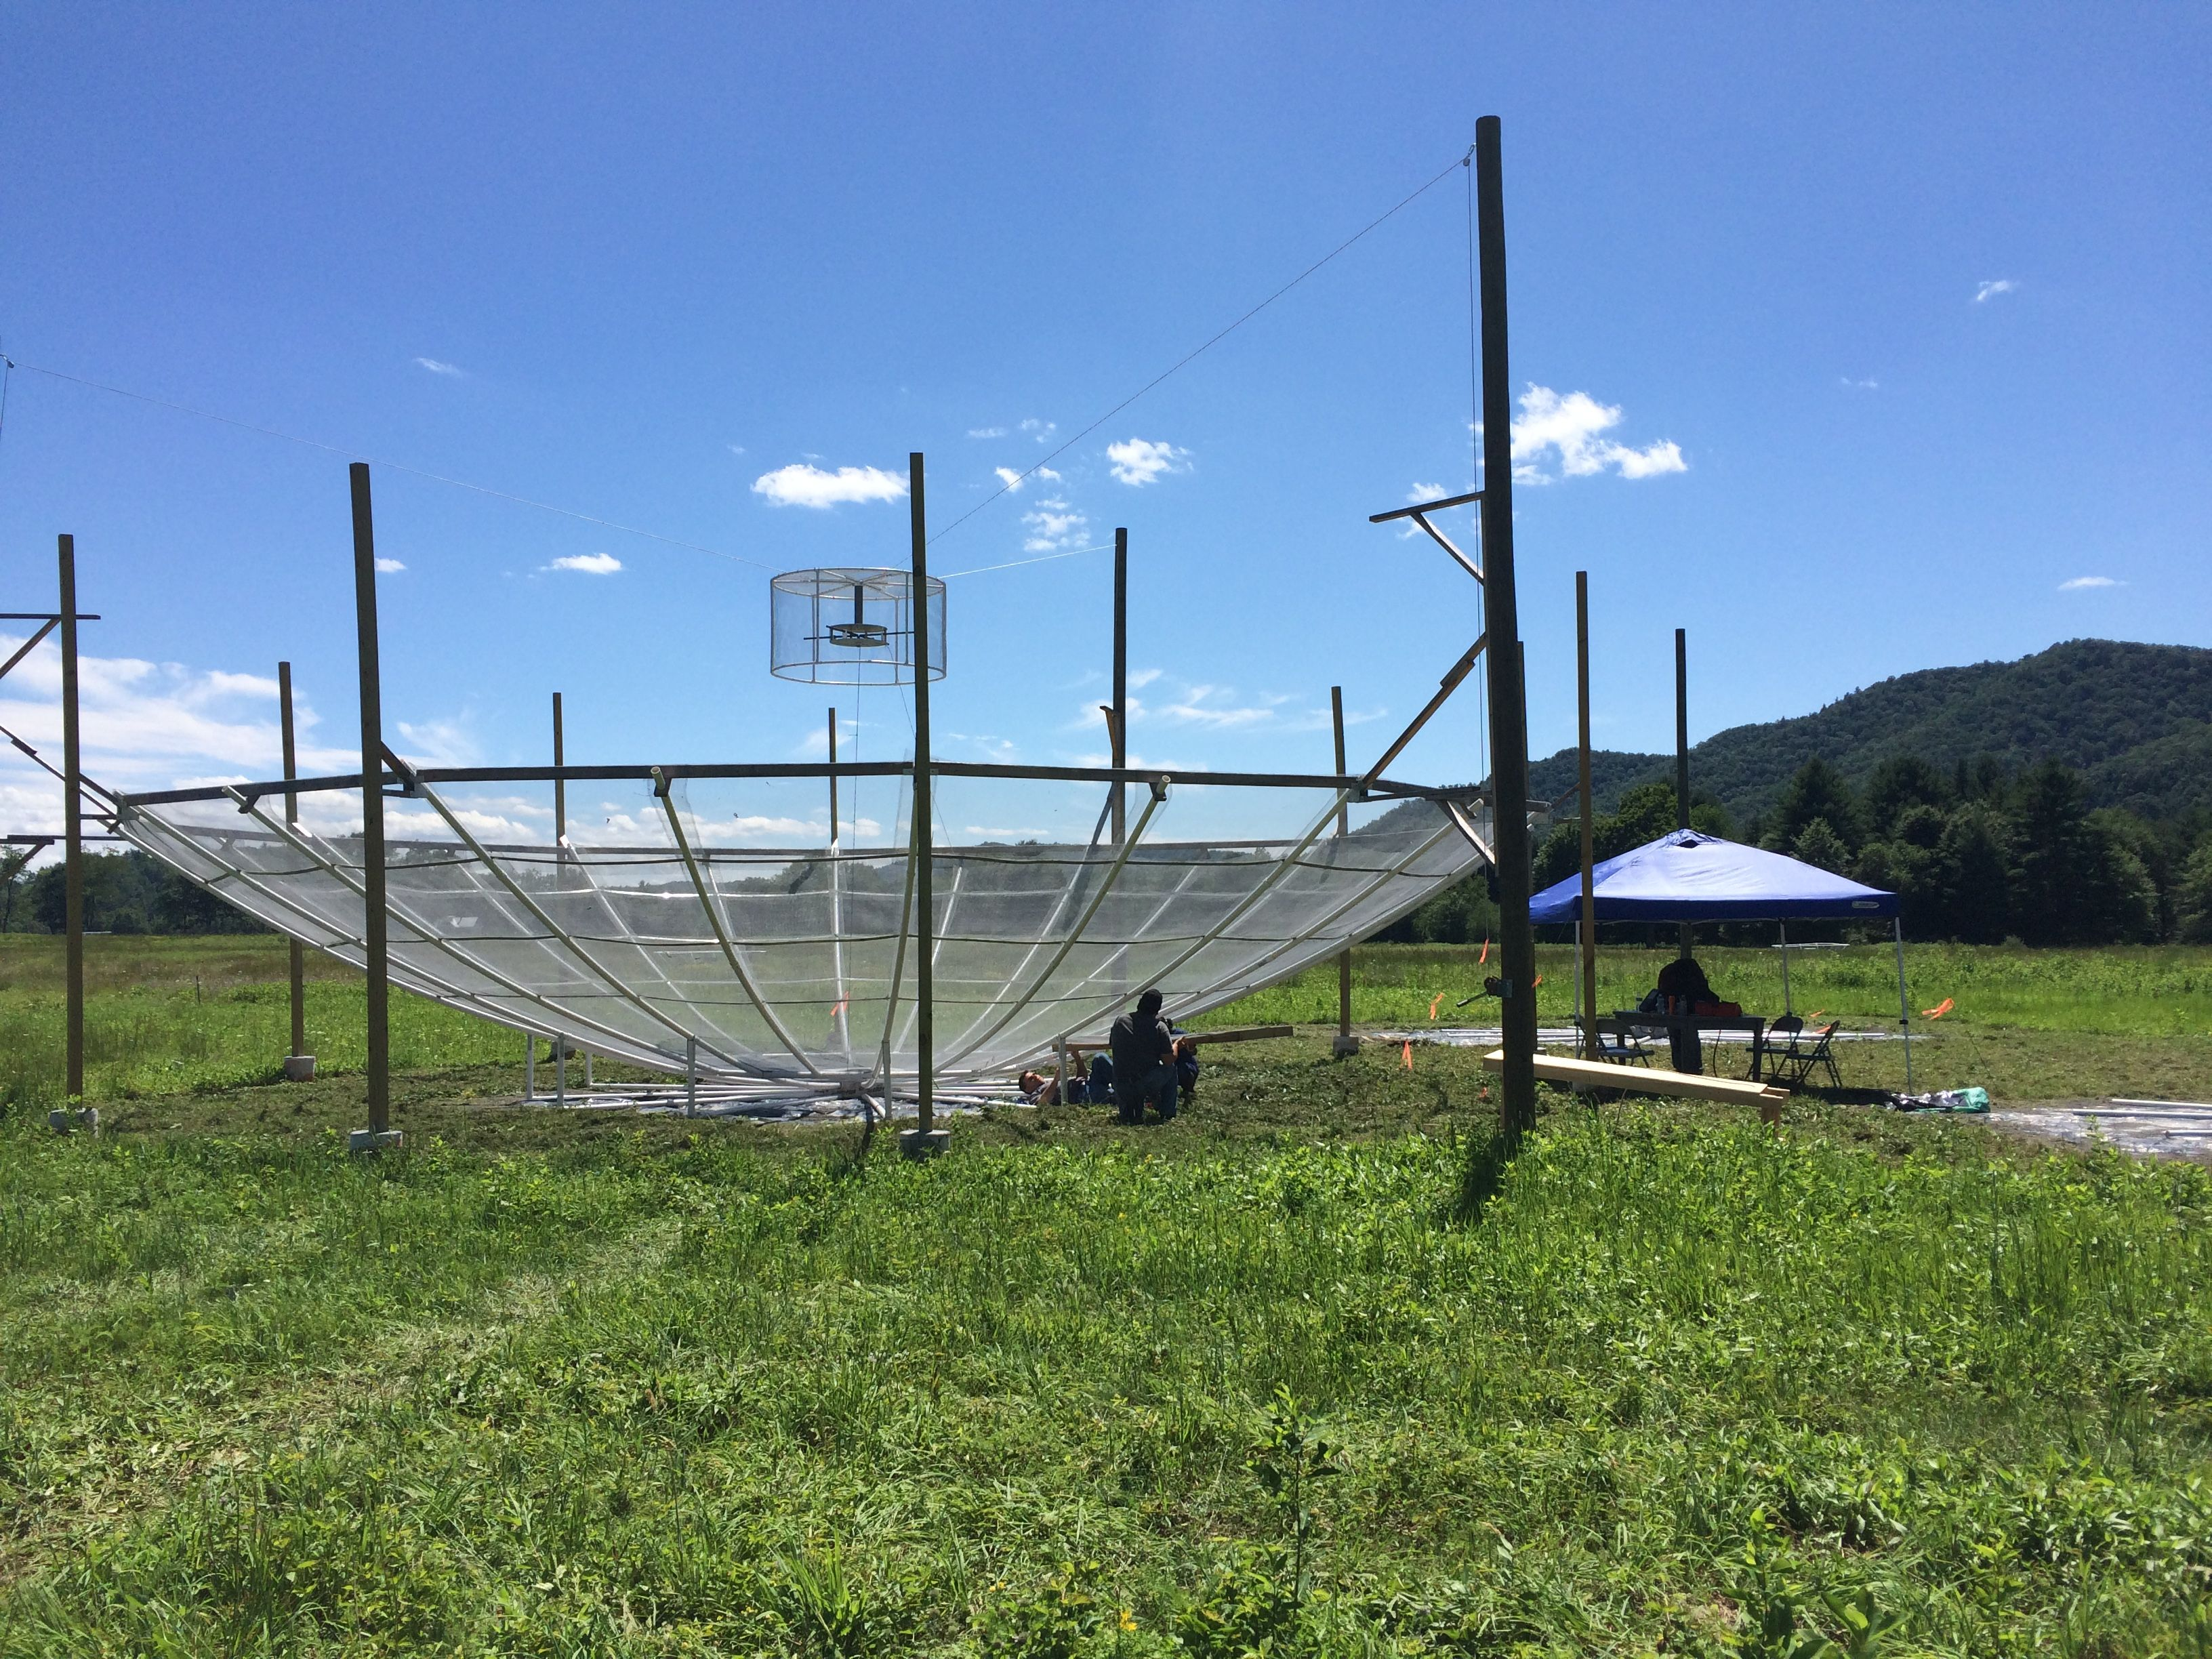
\includegraphics[trim={2cm 20cm 30cm 15cm},clip, totalheight=0.3\textheight]{plots/heradish.jpg}
\caption{HERA dish feed at the Green Bank NRAO site.}
\label{fig:heradish}
\end{figure*}


\section{\textbf{Visibility measurements by a two element interferometer and the delay spectrum}}
Consider a two element interferometer with a baseline $\vec b$. If we denote the electric field sky signal in the direction $\thhat$ by $\volt_\sky(\vec \theta, \nu)$, then the voltage output of each antenna may be written as,  

\begin{equation}
\volt_{1}(\thhat, \nu) = \bmvolt_{1}(\thhat,\nu)\volt_\sky(\thhat,\nu)\nonumber\\
\end{equation}
\begin{equation}
\volt_{2} (\thhat, \nu)= \bmvolt_{2}(\thhat,\nu)\volt_\sky(\thhat,\nu)\fngexp\nonumber\\
\end{equation}
Hence, the time averaged visibility measured by the interferometer may be written as, 
\begin{equation}
\vis(\vec b, \nu) =  \int  \volt_{1}(\thhat,\nu)  \volt_{2}^{*} (\thhat, \nu) \ifngexp d\Omega 
\label{eq1}
\end{equation}

We define the antenna cross power pattern as  $\beam(\thhat,\nu)=\bmvolt_{1}(\thhat,\nu)\bmvolt_{2}^{*}(\thhat,\nu)$ and denote the sky intensity as  $I_\sky(\thhat,\nu)=\volt_\sky(\thhat,\nu)\volt_\sky^{*}(\thhat,\nu)$. Hence, 
\begin{equation}
\vis(\vec b,\nu) = \int \beam(\thhat, \nu) I_\sky(\thhat,\nu) \ifngexp d\Omega
	%	& = & \int B(l,m, \nu) I_{sky}(l,m,\nu) exp(-2\pi i \nu \tau_{g} ) dl dm \nonumber\\
 	%	& = & B(\vec u,\nu) \ast P_{sky}(\vec u,\nu ) \nonumber\\
	%	& = & B(\nu { |\vec b| \over c} , \nu) \ast P_{sky}(\nu { |\vec b| \over c} , \nu) \nonumber\\
	%	& = & B(\tau_{g}, \nu) \ast P_{sky}(\tau_{g} , \nu)	
\label{eq2}
\end{equation}

%i.e, the complex visibility is the Fourier transform of the product of the antenna beam pattern with the sky angular power spectrum. In other words, it is the convolution of the Fourier transform of the antenna power pattern with the Fourier transform of the sky. The complex visibility measured by an interferometer with a given baseline length has explicit dependence on frequency as well as implicit frequency dependence through the spatial frequency $\vec u = \nu { \vec b \over c}$ component. Since $\vec u $ is the For a given baseline length $|\vec b|$, the visibility measured at various frequencies are not only the function of frequencies but also samples different $\vec u$ in the uv space. Delay transformation technique takes the visibility measurements at different frequencies and Fourier transforms the complex visibilities. If we defineI_{sky} the Fourier conjugate of the frequency axis as $\tau$ then the equation could be written as, 
In ~\citet{parsons_et_al2012a}, the Fourier transform of the visibility along the frequency axis was introduced,
resulting in the delay spectrum:
\begin{eqnarray}
\tilde V(\vec b, \tau) & = & \int\!\![{\beam(\vec b,\nu)*I_\sky(\vec b,\nu)] ~e^{-2\pi i\nu\tau}d\nu}%\nonumber\\	                        %& = &   \left [ A(\vec b, \tau)\ast I_{sky}(\vec b, \tau) \ast \delta( \tau - \frac{{\vec {b} \cdot \thhat}}{c} )\right ] d\Omega 
\label{eq3}
\end{eqnarray}
% XXX rethink how to express this equation (not correct about integrated over all sky)
% XXX define tau_g
The convolution is carried out along the $\tau$ axis which is Fourier conjugate of the frequency $\nu$. 
The redshifted 21 cm spatial power spectrum is defined as
\begin{equation}
  P(k_\perp,k_\parallel) = (|\tilde V(\vec b, \tau)|^{2} \left(\frac{1}{\Omega\Delta B}\right)\left(\frac{D^2\Delta D}{\Delta B}\right)\left(\frac{\lambda^2}{2k_\textrm{B}}\right)^2 ,
\label{eq:delay-power-spectrum}
\end{equation}
where
\begin{equation}
  k_\perp = \frac{2\pi f}{D}\Bigg({b\over c}\Bigg), \text{ }
  k_\parallel = \frac{2\pi\tau\,f_{21}H_0\,E(z)}{c(1+z)^2}, 
\end{equation}
The power spectrum is a function of cosmological as well as instrumental parameters which are:\\
$f_{21}$:rest frame frequency of the 21~cm radiation.\\
$f$: observation frequency.\\
$z$: cosmological redshift corresponding to the frequency of observation.\\
 $\Delta B$: bandwidth centered at the observation frequency.\\
 $k_\textrm{B}$: Boltzmann constant.\\
 $D\equiv D(z)$ comoving distance along the line of sight\\
 $\Delta D$ the comoving distance along the line of sight corresponding to bandwidth of observation $\Delta B$.\\
$E(z)= [\Omega_\textrm{M}(1+z)^3+\Omega_\textrm{k}(1+z)^2+\Omega_\Lambda]^{1/2}$ \\
\indent In this paper, we use $\Omega_{M}=0.27$, $\Omega_{\Lambda}=0.73$, $\Omega_{K}=1-\Omega_{M}-\Omega_{\Lambda}$, $H_0=100 h^{-1}\,$km$\,$s$^{-1}\,$Mpc$^{-1}$, and $P(k_\perp,k_\parallel)$ is in units of K$^2 (h^{-1}$~Mpc$)^3$.

\indent Since both $k_{\perp}$ and $k_{\parallel}$ are functions of the delay $\tau$, corresponding to the given baseline length, the redshifted 21 cm power spectrum could be estimated from the delay spectrum of the visibility measured by an interferometer. The sky delay spectrum from any direction $\thhat$ is convolved with the delay spectrum of the instrument and would be located at the delay $\tau = {\vec b \cdot \thhat \over c}$ %defined this differently earlier
 in the delay domain. The maximum geometric delay possible for a given baseline would be $\tau_{g} ={ b \over c }$ for the direction of $\thhat = 0$, when the phase centre is halfway in between the two antennas. %The phase center is elsewhere defined as being at the center of one of the antennas.
 Hence, the sky contribution from any direction would be confined within $-\tau_{g}<\tau<\tau_{g}$. Due to the chromaticity of the sky signal as well as the instrument response, the delay spectrum of the sky spills over into delays with $\tau> \tau_{g}$, with a decaying amplitude [Ref to the Figure Parsons12]. The foreground, $P_{fg}(\tau)$, which is spectrally smooth, and the 21~cm power spectrum, $P_{21}(\tau)$, which contains spectral signatures, contribute to the sky delay spectrum $P_{sky}(\tau)$.Therefore, in the spill over region $(\tau>\tau_{g})$, the relative strength of the smooth spectrum foreground, with respect to the delay spectrum of the $I_{21}$, reduces and the 21cm delay spectrum could be detectable.

 %In words, the sky delay spectrum from any direction $\thhat$ is convolved with the delay spectrum of the instrument and would be located at the delay $\tau = {\vec b \cdot \thhat \over c}$ in the delay domain. The maximum geometric delay possible for a given base line would be $\tau_{g} ={ b \over c }$ for the direction of $\thhat = 0$ when the phase centre is halfway in between the two antennas. Hence, the sky contribution from any direction would be confined within $-\tau_{g}<\tau<\tau_{g}$. Due to chromaticity of the sky signal as well as instrument reponse, the delay spectrum of the sky spills over the delay $\tau> \tau_{g}$ with decaying amplitude [Ref to the Figure Parsons12]. Sky delay spectrum $I_{sky}(\tau)$ is contributed by the foreground  $I_{fg}(\tau)$  which is spectrally smooth and the 21~cm power spectrum $I_{21}(\tau)$ which contains spectral signatures. Therefore, in the spill over region $(\tau>\tau_{g})$, the relative strength of the smooth spectrum foreground with respect to the delay spectrum of the $I_{21}$ reduces and the 21~cm delay spectrum could potentially be detectable. 


%\subsection{Delay spectrum: An estimate of the 21cm power spectrum}
%Add text here. 
 %\textbf{[ Reference to Nithya's foreground simulation work, reference to any plots on the relative contribution of the  foreground and EoR signal. ]}

\section{\textbf{Effects of multiple reflections on visibility and delay spectrum}}
The Hydrogen Epoch of Reionization Array consists of parabolic dishes which provide increased collecting area per array element compared to its predecessor experiment PAPER. Plane waves incident on a parabolic dish are focussed at the feed which is kept at the focal plane of the dish.
The mismatch between the impedance of free space and the feed and transmission line results in a partial coupling of the sky signal into the feed while the rest is reflected off the feed. 
The reflected signal illuminates the dish and most of it is reflected back into the space.
However, a part of it reflects back and forth several times in between the feed and the vertex of the dish which is shadowed by the feed (dashed blue arrows in Figure \ref{fig:cartoon}).
Such reflections generate multiple copies of the incident sky signal of reduced strength at various delay and phase and thus produces spurious correlations in the visibilities of interferometric data.  Identical spurious visibilities could be resulted due to reflections internal to the system causing delay space distortion. Therefore, it is necessary to measure and understand the instrument delay spectrum in order to qualify the system for the measurement of 21cm power spectrum. 
In this section we compute the visibility of a two element interferometer accounting for the additional reflections of the sky signal in between the feed and the dish vertex and the corresponding effects on the delay spectrum, using the multiple reflection formulation of Sec. \ref{sec:multiple}. In this section, the effect of reflections on the visibility data and corresponding effect on the delay spectrum is discussed in detail. We assume two antennas with identical geometry and electrical parameters i.e, $\bmvolt_{1}(\thhat,\nu)=\bmvolt_{2}(\thhat,\nu) = \bmvolt(\thhat,\nu)$. 
 \subsection{\textbf{Antenna Reception With Multiple Reflections}}
\label{sec:multiple}
To examine the performance of an antenna and feed in the presence of multiple reflections, we can think of the system as a screen at a distance $F$ from a feed (see Figure \ref{fig:sys}), noting that this does ignore the sky pattern of the feed itself.  The screen reflects a factor, $\Gamma_d$, of the voltage and transmits $(1+\Gamma_d)$ (see, {\em e.g.} Pozar).  Similarly, the feed reflects $\Gamma_f$ and transmits $(1+\Gamma_f)$.  The voltage pattern $\volt_{sky}$ is incident onto that system and  $(1+\Gamma_{d})(1+\Gamma_{f})$ is coupled into the cable leading from the feed. 
Additionally, however, the voltage pattern is reflected off the feed ($\Gamma_f$), then the dish ($\Gamma_d$) and subsequently $(1+\Gamma_{f})$ of it reenters the feed with a roundtrip time delay $\Delta \tau=2F/c$. Hence, if $v_{sky}$ is reflected $n$ times in between the feed and the dish, the net voltage entering the feed after the
$n^{th}$ reflection may be written as:
\begin{eqnarray}
\volt_{rec} & = &  (1+\Gamma_d) (1+\Gamma_{f}) \volt_{sky}[1+ \Gamma_{f}\Gamma_{d} \dfngexp \nonumber \\
	&& + (\Gamma_{f}\Gamma_{d})^2  (\dfngexp)^{2}+ \nonumber \\
&&  ....+ (\Gamma_{f}\Gamma_{d})^{n} (\dfngexp)^{n}]
\end{eqnarray}
\begin{figure}
\centering
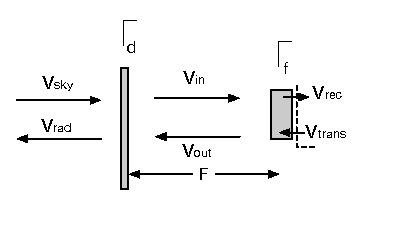
\includegraphics[width=0.5\textwidth]{plots/microsys.pdf}
\caption{System}
\label{fig:sys}
\end{figure}

\noindent
%Defining $a=\volt_{rec}/\volt_{sky}$ and we see that 
Hence,
 \begin{eqnarray}
{\volt_{rec}\over \volt_{sky} } & = &   (1+\Gamma_d)(1+\Gamma_{f}) \displaystyle\sum\limits_{n=0}^{N} [\Gamma_{f}\Gamma_{d}\dfngexp]^{n}\nonumber\\
& = & \frac{ (1+\Gamma_d)(1+\Gamma_{f})}{1+\Gamma_{f}\Gamma_{d}\dfngexp} 
\label{corrected_response}
\end{eqnarray}
Note that $n=0$ is when the initial wave enters the cable at the feed (where we assume we have set our reference plane).  We may identify $(1+\Gamma_d)$ as the voltage reception pattern of the antenna, denoted $\bmvolt(\thhat,\nu)$, which is a function of angle on the sky.  Additionally, $(1+\Gamma_f$) is the voltage efficiency for the feed (not a function of angle).

%As an aside, note that the sum in Eq. \ref{eq:Sigma} may be evaluated we may rewrite
%\begin{equation}
%{\volt_{rec}\over \volt_{sky} } =  (1+\Gamma_d)(1+\Gamma_{f})\frac{1+\Gamma_{f}^{N+1}\Gamma_{d}^{N+1}(\dfngexp)^{N+1}}{1+\Gamma_{f}%\Gamma_{d}\dfngexp} \nonumber
%\end{equation}
%which, in the limit becomes:
%\begin{equation}
%{\volt_{rec}\over \volt_{sky} } = \frac{ (1+\Gamma_d)(1+\Gamma_{f})}{1+\Gamma_{f}\Gamma_{d}\dfngexp} \nonumber
%\end{equation} 
%since $|\Gamma_d|$ and $|\Gamma_f|$ are less than one.

An accurate measurement of this quantity requires receiving $v_{sky}$ from a well calibrated, wideband source in the sky in the far field of the HERA antenna element with significant isotropic emission. While this condition is hard to achieve in practice, due to the reciprocity of the antenna performance in the transmission and reception mode, the right hand side of equation \ref{eq:Sigma} could be measured using the return loss measurement technique with a vector network analyzer (VNA). \\
\section{\textbf{Reflectometry measurements}} 

Reflectometry measurements are carried out at the HERA element prototype in Green
Bank, WV (Figure \ref{fig:heradish}) in order to measure the instrument response of the feed and dish assembly and characterise the performance.  HERA element consists off a $14\,m$ diameter
parabolic reflector and a crossed-dipole pair as a feed. The cross dipole antenna pair is identical to the feed of the PAPER antenna which is suspended at the focal plane of the dish with the support of three vertical poles. HERA elements are closely spaced with centre to centre distance between two dishes are equal to the dish diameter. Therefore, to reduce the coupling between the adjacent dishes, the crossed dipole feed along with the back plane is encased in a cylindrical cage. The feed is raised and
lowered by a three-pulley system mounted on the three poles. The focal height of the dish is $5m$.  The detail geometry and electromagnetic design of of the feed is presented in deBoer et al 2016. \\
%A vector network analyser is connected via a 50feet long cable at the feed output of the HERA element and the return loss $(s_{11})$ of the HERA element is measured as a function of frequencies while the feed is suspended at the focal plane of the dish. 

 A VNA is connected to the HERA element via a 50-foot cable. It then transmits a broadband noise voltage, $\volt_{trans}$, and a factor $(1+\Gamma_f)$ of this voltage is radiated by the feed while the fraction $\Gamma_{f}$ returns to the VNA. Although the radiated signal illuminates the dish and most of it is radiated into free space, a fraction $\Gamma_d$ of this signal is reflected back towards the feed, and $(1+\Gamma_f)$ is received by the VNA.  The received voltage, after $n$ reflections between the dish and the feed (where again $n=0$ is the first reflected signal at the reference plane), is therefore:

\begin{eqnarray}
\volt_{rec} & = &  \Gamma_f \volt_{trans} \nonumber \\
         && + \volt_{trans} (1+\Gamma_f)^2 \Gamma_{d} \dfngexp \nonumber \\
         && + \volt_{trans} (1+\Gamma_f)^2 \Gamma_{d} \dfngexp \Gamma_d\Gamma_f\dfngexp \nonumber \\
         && + \volt_{trans} (1+\Gamma_f)^2 \Gamma_{d} \dfngexp (\Gamma_d\Gamma_f\dfngexp)^2 \nonumber \\
&&  ....+ \volt_{trans} (1+\Gamma_f)^2 \Gamma_{d} \dfngexp (\Gamma_d\Gamma_f\dfngexp)^n \nonumber \\
\end{eqnarray}
Therefore, 
\begin{equation}
{\volt_{rec}\over \volt_{trans} } = \Gamma_f + \frac{(1+\Gamma_f)^2}{\Gamma_{f}} \displaystyle\sum\limits_{n=1}^{N} [\Gamma_{f}\Gamma_{d}\dfngexp]^{n}
\label{eq:s11}
\end{equation}
The VNA measures the quantity $\volt_{rec}/\volt_{trans}=s_{11}$ which is the voltage reflection coefficient of the HERA element.
The fundamental differences between the right hand side of equations \ref{eq:Sigma} and \ref{eq:s11} are the $n=0$ term and the multiplicative factor in front of the convergent series $\displaystyle\sum\limits_{n=1}^{N} [\Gamma_{f}\Gamma_{d}\dfngexp]^{n}$ that represents the contribution of the delayed voltage components at the VNA input, arising due to multiple signal reflections between the feed and the dish. Finally, writing $\volt_{rec}/\volt_{trans}=s_{11}$, equation \ref{eq:s11} can be written as,
\begin{equation}
s_{11} +\frac{(1+\Gamma_f)^2}{\Gamma_f}-\Gamma_f = \frac{(1+\Gamma_f)^2}{\Gamma_{f}} \displaystyle\sum\limits_{n=0}^{N} [\Gamma_{f}\Gamma_{d}\dfngexp]^{n}
\end{equation}
Comparing to Eq. \ref{eq:Sigma} and we find that
\begin{eqnarray}
{\volt_{rec}\over \volt_{sky} } & = & (1+\Gamma_d)\left[(1+\Gamma_f) + \frac{\Gamma_f}{(1+\Gamma_f)}\left(s_{11} - \Gamma_f\right)\right] \nonumber\\
 & = & \bmvolt(\thhat,\nu) \left[(1+\Gamma_f) + \frac{\Gamma_f}{(1+\Gamma_f)}\left(s_{11} - \Gamma_f\right)\right]
\label{zero_delay_correction}
\end{eqnarray}
When the feed return loss is measured separately, all the higher order terms of equation \ref{eq:s11} do not exist. In this case, $\Gamma_f = s_{11}^{f}$. Using this measurement and the VNA measurement of $s11$, the quantity $v_{rec}\over v_{sky}$ is estimated. \\
%
\indent From this, for a two element interferometer with identical antenna elements, the ratio of the received sky intensity to true sky intensity will be, 
\begin{eqnarray}
{I_{rec}\over I_{sky} } & = & \Bigg|{\volt_{rec}\over \volt_{sky} }\Bigg|^2 =  \beam(\thhat,\nu)\times \nonumber\\
             && \left[|1+\Gamma_f|^2 +  2\operatorname{Re}\left(\frac{\Gamma_f}{(1+\Gamma_f)}(s_{11} - \Gamma_f)\right)\right] + \nonumber\\ 
             &&  \left[ \frac{|\Gamma_f|^2}{|1+\Gamma_{f}|^2}|s_{11} - \Gamma_f|^2  \right]  \nonumber\\
\label{eq:power_ratio}             
\end{eqnarray}

In terms of visibility, the same could be written as,  
\begin{eqnarray}
\vis^{mul}(\vec b,\nu) & = & \int \beam(\thhat,\nu)\times \nonumber\\
             && \left[|1+\Gamma_f|^2 +  2\operatorname{Re}\left(\frac{\Gamma_f}{(1+\Gamma_f)}(s_{11} - \Gamma_f)\right)\right] + \nonumber\\ 
             &&  \left[ \frac{|\Gamma_f|^2}{|1+\Gamma_{f}|^2}|s_{11} - \Gamma_f|^2  \right]  I_{sky} \ifngexp d\Omega
\label{visibility_mul}
\end{eqnarray}

Comparing equations \ref{eq:power_ratio} and \ref{eq2}, the cross power generated by $v_{1}$ and $v_{2}$ would have a spurious visibility response due to the mutual correlation between multiply reflected voltages represented by the second and the third term of the right hand side of equation \ref{eq:power_ratio}. In the ideal case, $\Gamma_{f}=0$, in which case equation \ref{eq:power_ratio} results in equation \ref{eq2}. The Fourier transform of this visibility spectrum along the frequency axis results in the delay spectrum. 
In the delay domain, visibilities contributed to by any two voltage components from two antennas with no mutual delay will be located at the delay $\tau = 0$ whereas any two voltage components from two antennas having a mutual delay of $n\Delta \tau$ will be centred at $n\Delta \tau$. These will broaden the width of the delay spectrum, which ultimately interferes with the 21cm power spectrum detection.

\begin{figure*}
\centering
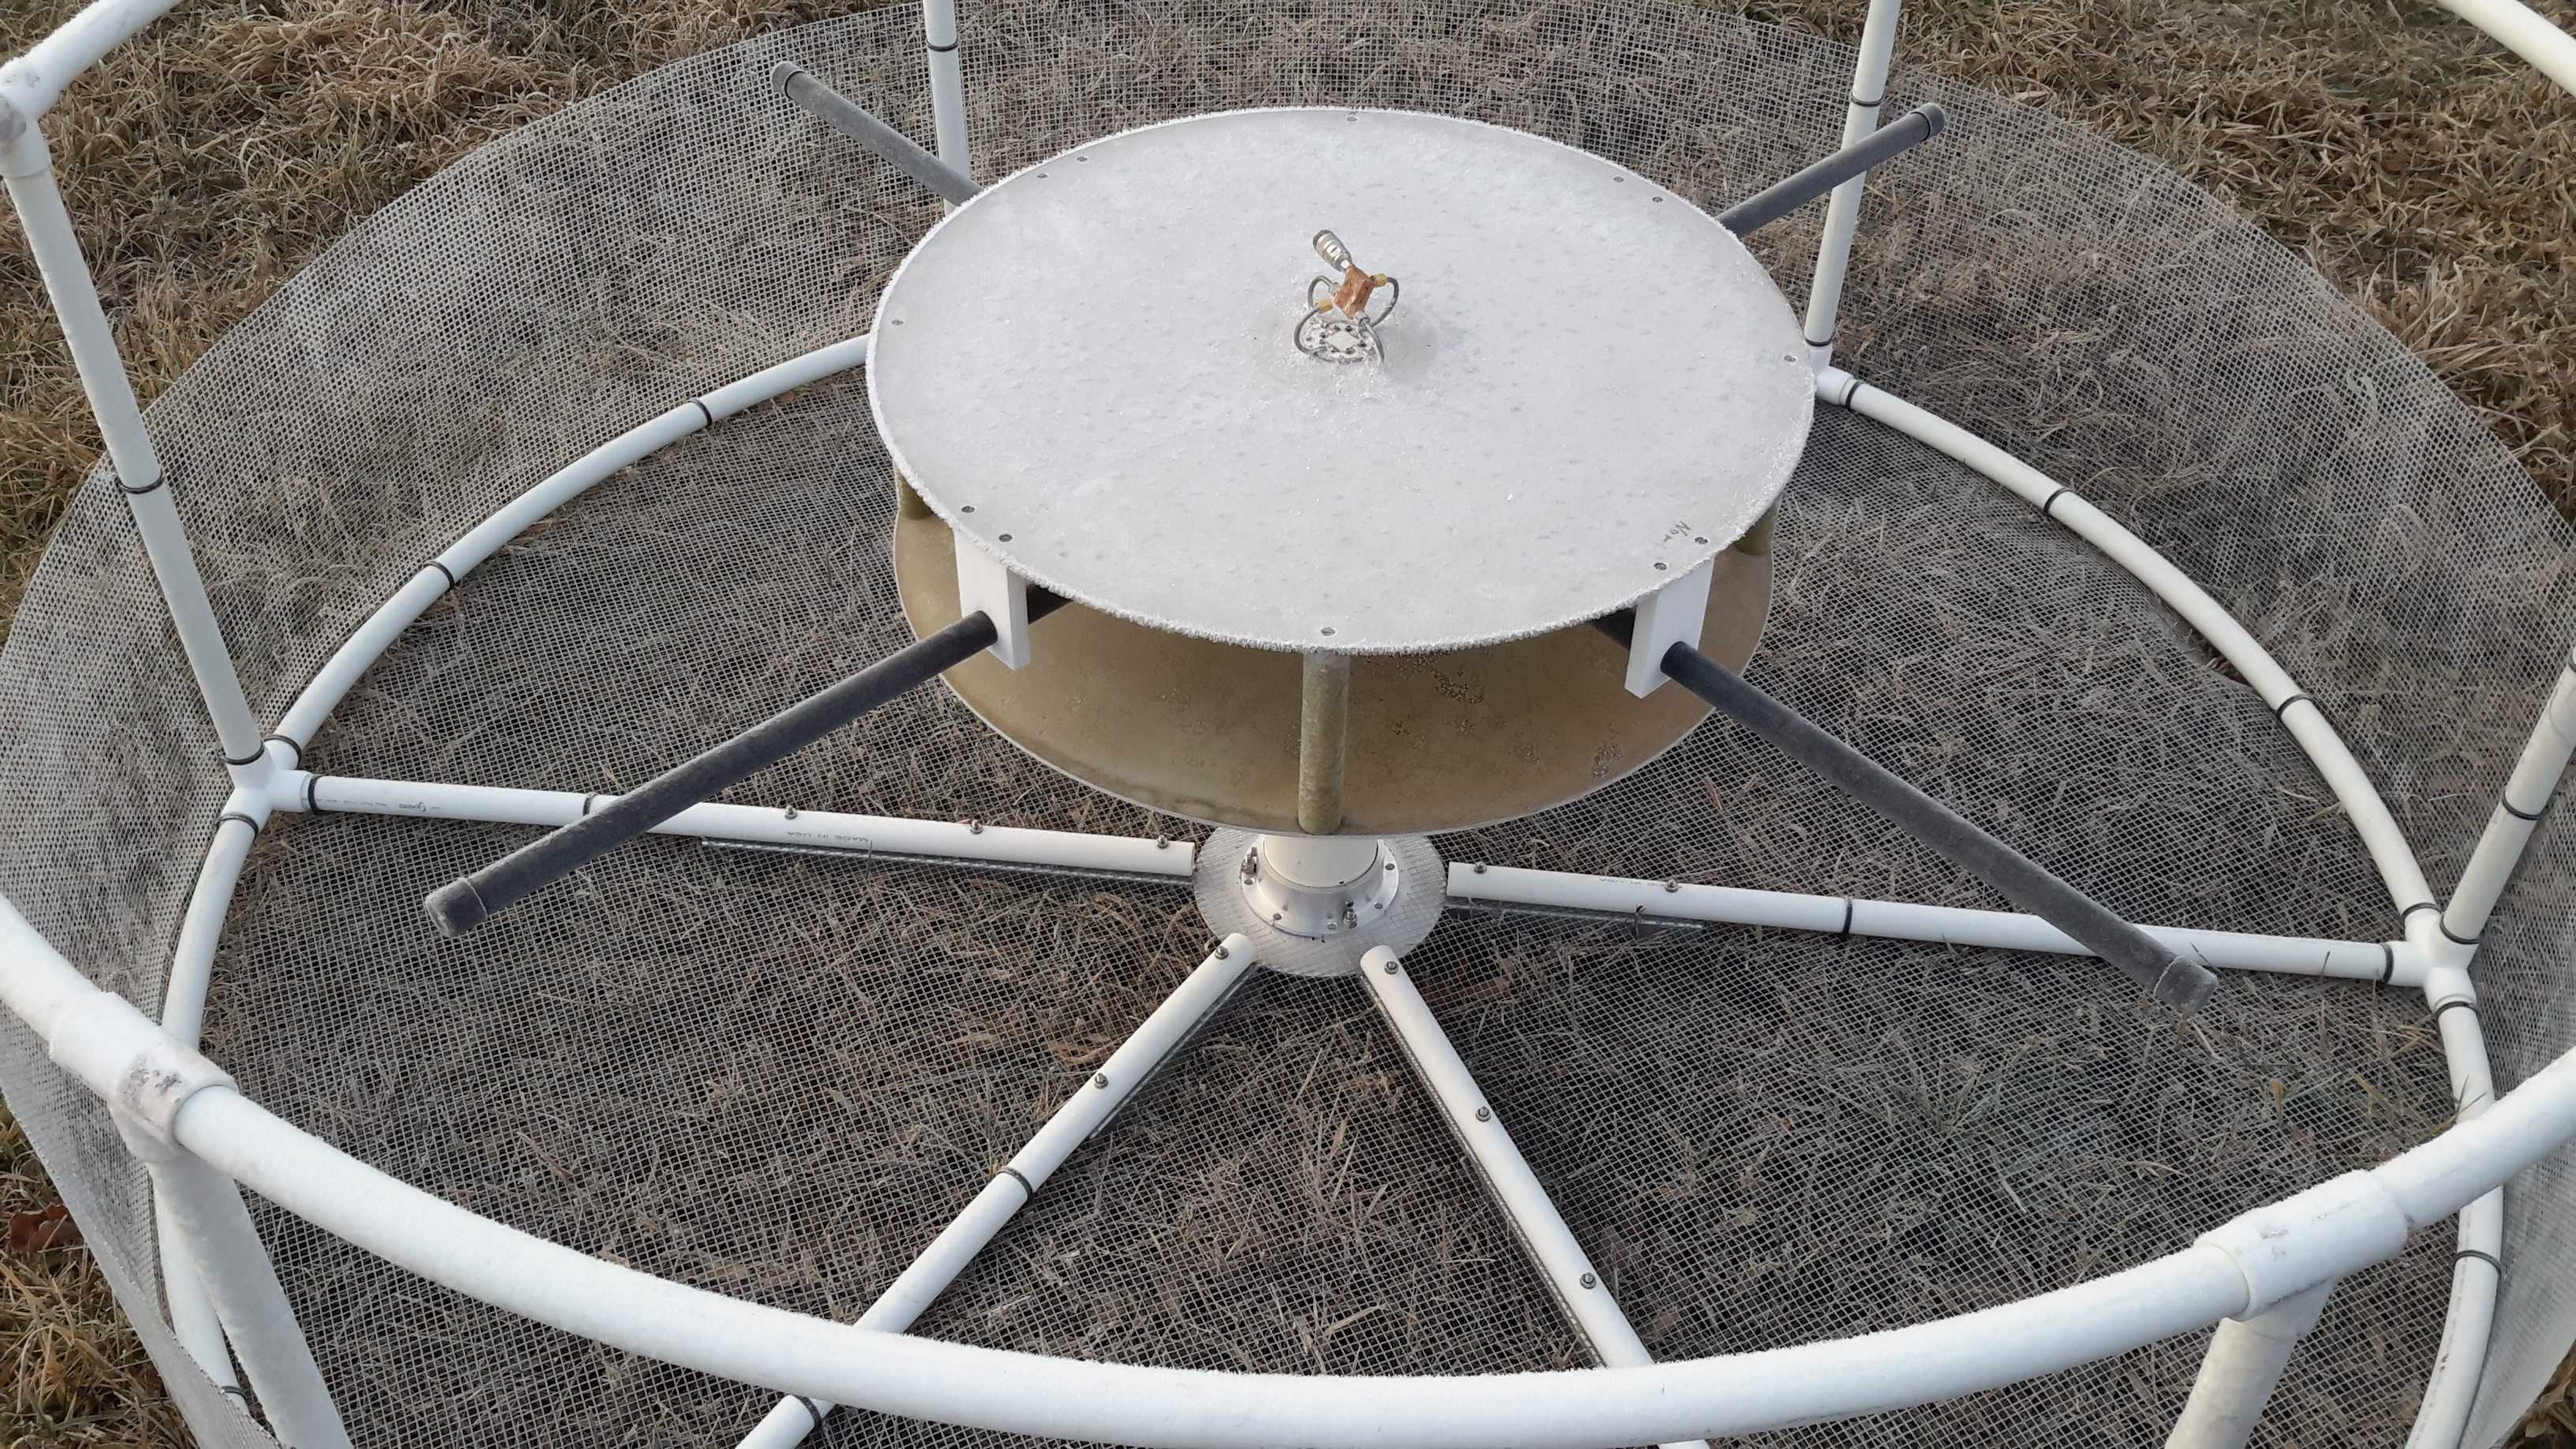
\includegraphics[trim={2cm 10cm 20cm 5cm},clip, totalheight=0.3\textheight]{plots/herafeed.jpg}
\vspace{1.0 em}
\caption{The HERA feed consists of a pair of crossed-dipoles ove xxx mt diameter backplane made of wire mesh. The backplane is surrounded by xxx m wire mesh around the edge resulting in encasing the crossed-dipoles in a cylindrical cage.}
\label{fig:herafeed}
\end{figure*}


Return loss measurements are similar to auto correlation measurement from a single HERA element. Upon our assumption that two adjacent antenna elements have identical design parameters and electrical properties, this power is also a measure of the cross power or the visibility $\vis (\vec b, \nu)$ between the two antennas with a normalisation factor of $2$. 

The simultated and measureded return loss of the feed as well as the HERA element is shown in figure \ref{meas_sim_RL_feed} and figure \ref{meas_sim_RL_HERA}.
\begin{figure}[ht]
\begin{minipage}[b]{\linewidth}
\centering
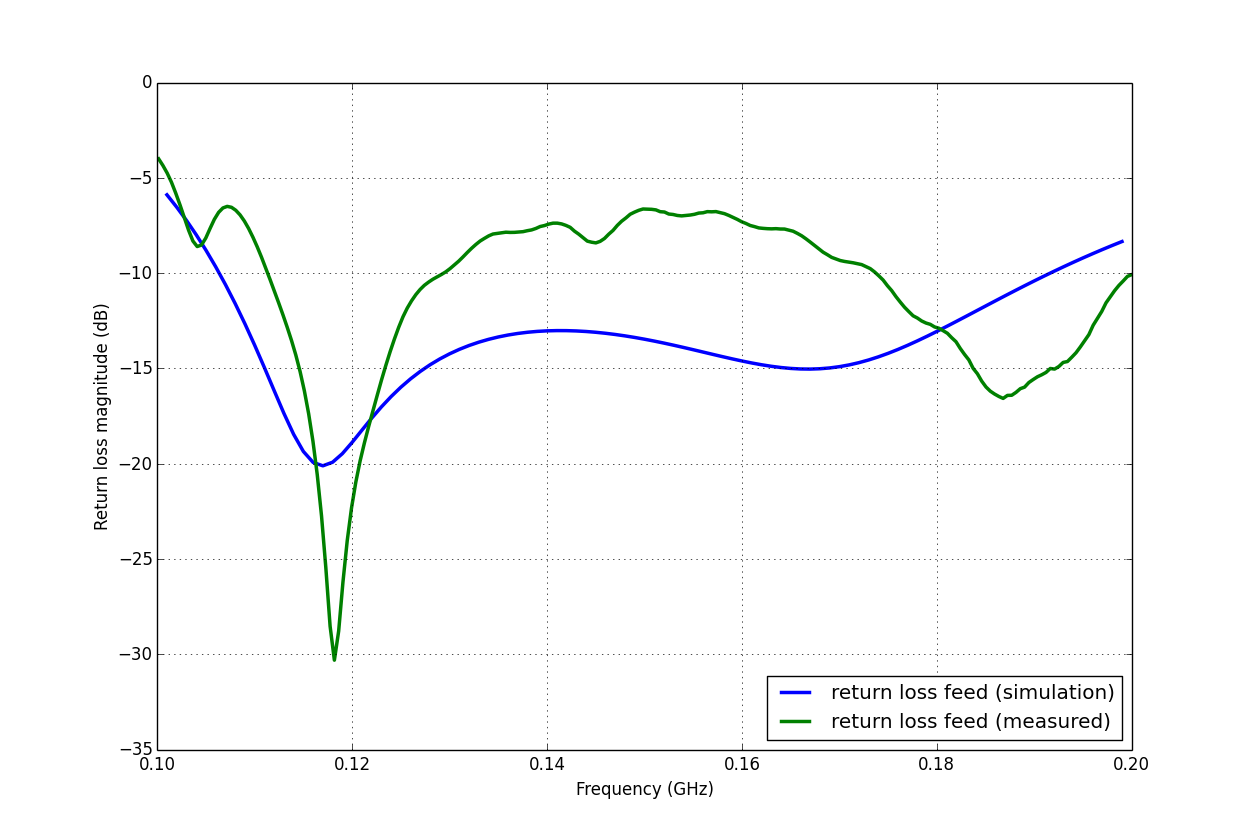
\includegraphics[angle=0, width=\linewidth]{plots/feed_meas_sim_mag.png}
\end{minipage}
\vspace{0.1cm}
\begin{minipage}[b]{\linewidth}
\centering
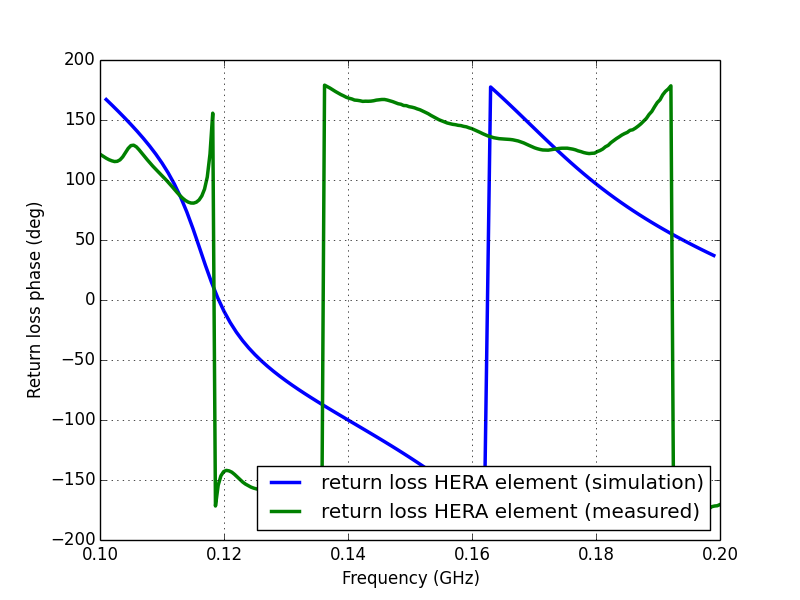
\includegraphics[angle=0, width=\linewidth]{plots/feed_meas_sim_ph.png}
\end{minipage}
\caption{Magnitude and phase of the return loss of the feed as simulated and measured. While both the measurement and the simulation shows similar resonance around $120~MHz$, the simulation shows a better matching to a 50 Ohm transmission line compared to the measurements. The measurement also has some small scale fluctuation due to multiple reflection of the signal at the VNA input. }   
\label{meas_sim_RL_feed}
\end{figure}



\begin{figure}[ht]
\begin{minipage}[b]{\linewidth}
\centering
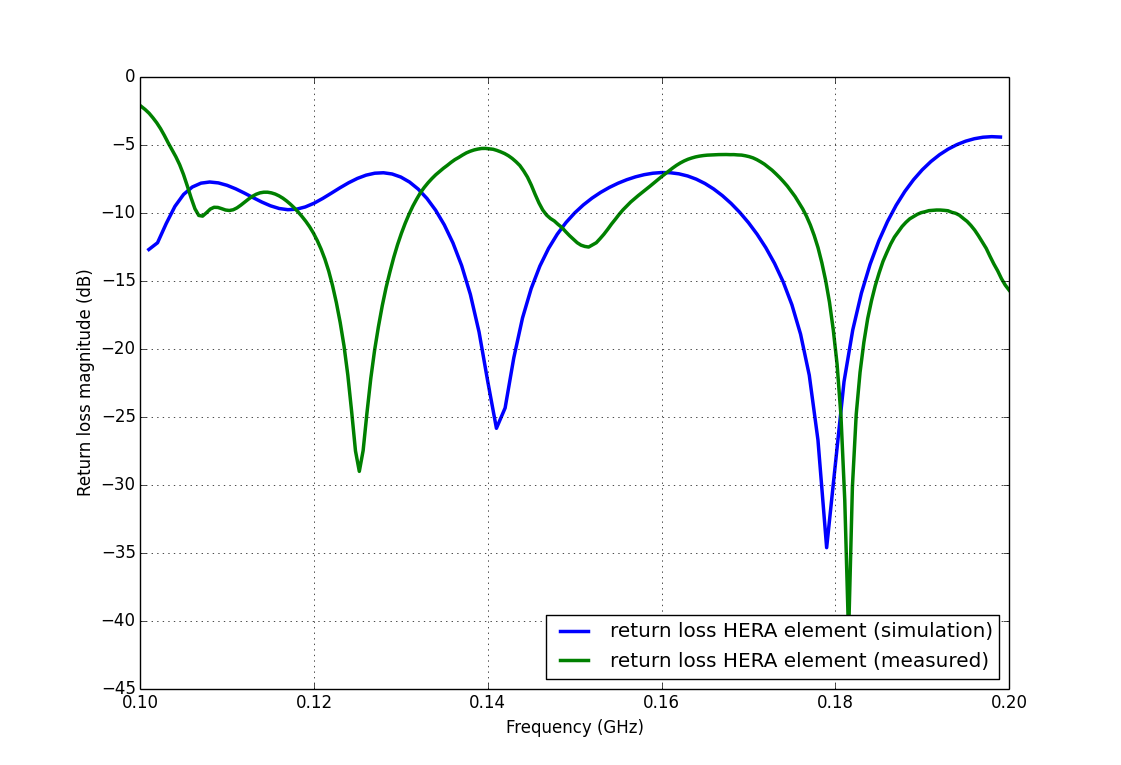
\includegraphics[angle=0, width=\linewidth]{plots/HERA_meas_sim_mag.png}
\end{minipage}
\vspace{0.1cm}
\begin{minipage}[b]{\linewidth}
\centering
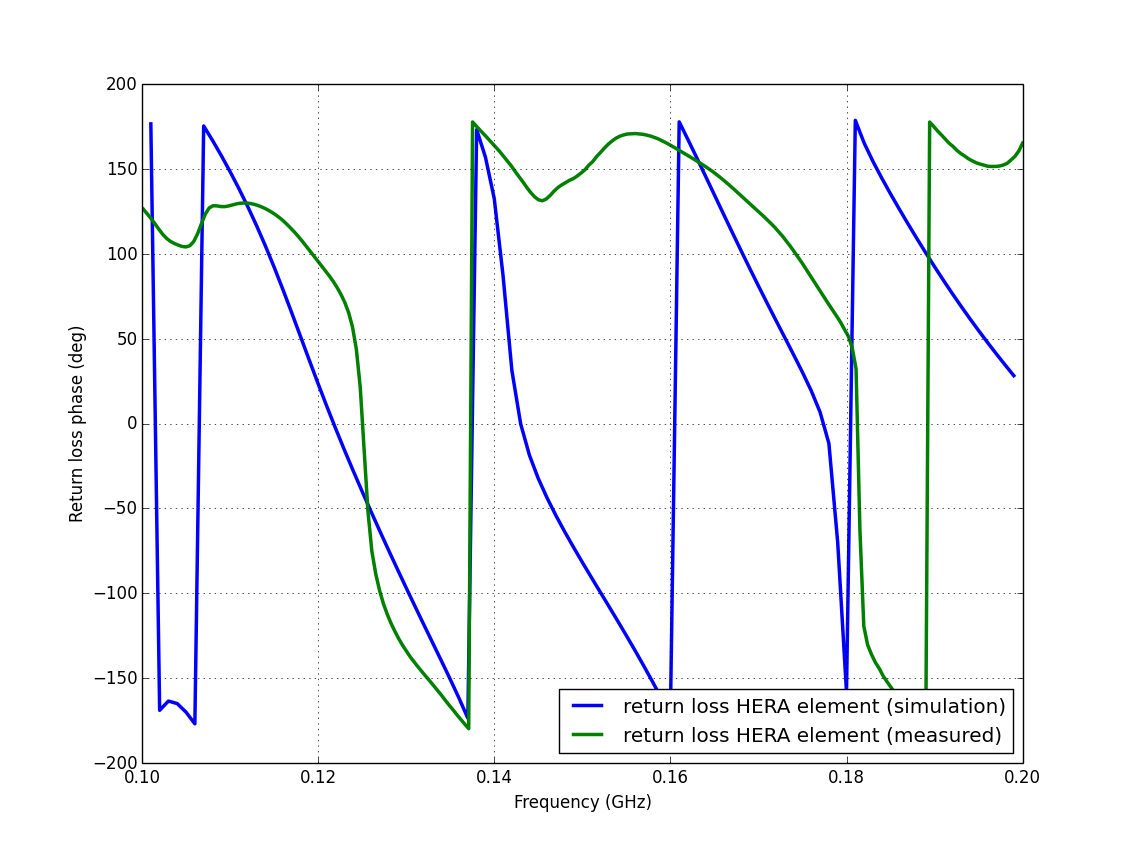
\includegraphics[angle=0, width=\linewidth]{plots/HERA_meas_sim_ph.png}
\end{minipage}
\caption{Magnitude and phase of the return loss of the HERA element as simulated and measured. In this case, both measurement and simulation shows similar level of return loss across the band with marginally better return loss at the high frequency end of the band. }   
\label{meas_sim_RL_HERA}
\end{figure}

\section{Results}
\begin{figure}       
\centering
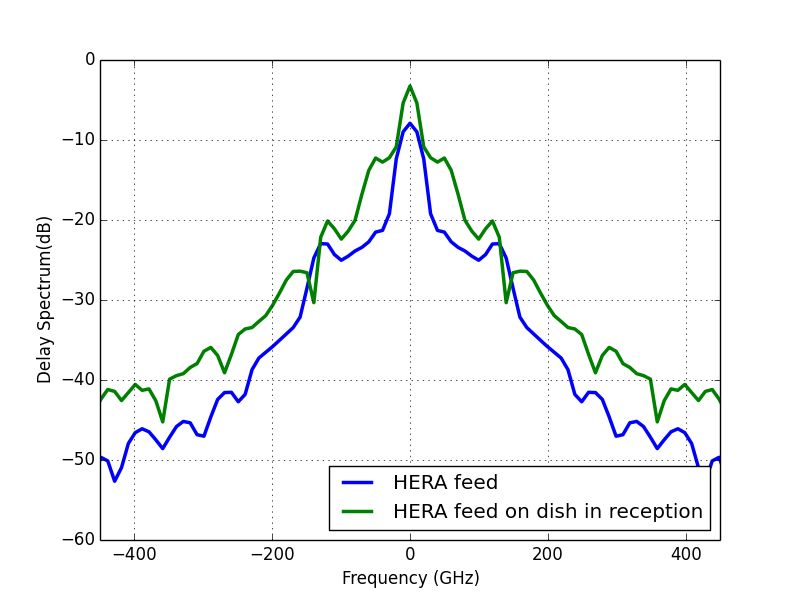
\includegraphics[width=\linewidth]{plots/H_dish_feed.png}
\caption{Delay spectrum of the HERA element (green) the HERA feed (blue) estimated by taking the Fourier transform of the measured return loss of power at the feed output. The feed, when suspended on the dish results in a more complex return loss and corresponding delay response is shown in the figure. After correcting the measurements from the transmission mode to reception mode by equation \ref{eq:power_ratio} the delay spectrum in the receiving mode is estimated (red). }
\label{fig:delay_spectrum}
\end{figure}

Figure \ref{meas_sim_RL_HERA} shows the return loss measured between $100$ to
$200MHz$ when the feed is suspended at the focal plane of the parabolic dish which is at $5m$ from the dish vertex. This measurement is first correc ted to map the response of the antenna from transmitting mode to receiving mode via equation \ref{zero_delay_correction}. The corrected measurement is then Fourier transformed to obtain the delay spectrum of the instrument in the receiving mode as given in equation \ref{corrected_response}. Measurement bandwidth is kept much larger than the bandwidth of operation to achieve higher delay resolution. A number of systematic effects as well as mathematical artefacts that are critical to this measurements and their effects on the corresponding estimation of the delay spectrum are taken in to account in determination of the delay spectrum and described below. 

\subsection{\textbf{Zero delay correction}}
%At first, the frequency domain measurement of s11 is Fourier-transformed to compute the response of the system in the delay domain. 

While measuring the return loss of the dish-feed assembly, the signal transmitted by the VNA is reflected first off the feed. This is represented by $\Gamma_{f}$ in equation \ref{eq:power_ratio}. This essentially represents a mismatch in between the feed and the 50 Ohm transmission line. In delay domain, this appears at the zero delay bin. The zero delay response is identical whether or not the feed is suspended on the dish. Therefore, we measure this response by measuring the feed return loss alone while the feed is kept on the ground facing the sky. This results in feed return loss alone including the surrounding cage structure but excluding the dish response. While $\Gamma_{f}$ fraction of incident voltage is reflected off the feed, $1+\Gamma_{f}$ fraction of the voltage is transmitted. In receiving mode, upon initial incidence, $\Gamma_{f}$ fraction of voltage is reflected back in to the space while $1+\Gamma_{f}$ voltage enters the feed. In receiving mode, in delay domain, this appears at the zero delay bin.
The using the return loss measurement of the feed $(\Gamma_{f})$, the return loss measurement $s_{11}$ of the dish and feed assembly is corrected via equation \ref{eq:power_ratio} and the quantity of interest ${I_{rec}\over I_{sky}}$ is estimated. 

\subsection{\textbf{Antenna beam pattern and feed return loss}}
The return loss $\Gamma_{f}$ determines the amount of power coupled to the system via the feed antenna. Additionally, with each reflections, the power coupled to the system reduces by a factor of $\Gamma_{f}^{2}$. Since reflected signal results in system response in higher delay, multiple reflections of the signal off the feed and the dish would result in an exponential envelope in the delay spectrum.  The return loss of power results from the antenna impedance mismatch with the free space as well as the transmission line. While antenna beam pattern $A_{f}$ is a smooth function of frequency and should have its imprint confined to lower delays, the return loss $\Gamma_{f}$ broadens the delay spectrum. However, a smaller return loss will result in vertical shift of the delay spectrum at lower values and therefore can make the higher order reflections insignificant. During observation, each HERA element is connected to an active balun similar to the ones used in the PAPER antenna (need reference) which provides greater than 10dB return loss of power at the feed output.These baluns are under further design improvements aiming at 10 to 20dB better imepedance match between the feed and the balun than the measurements presented here.  Our measurement is done using a vector network analyser for which the active balun has been replaced by a passive balun.Given the antenna impedance and the 50 Ohm transmission line the measurements are done using the passive balun with a 2:1 impedance ratio providing a net return loss of power between the sky, the antenna and the transmission line shown in the figure \ref{meas_sim_RL_feed}. This measurements are conservative estimate  for both $\Gamma_{f}$ and $s_{11}$.

\subsection{\textbf{Dish reflections}}
Measurement equations shows the effects of multiple reflections of the sky signal between the feed and the dish. Any other reflections off the feed structure and/or any other part of the dish-feed assembly would appear at arbitrary delays. The estimated delay spectrum of the instrument is collectively contributed by all the reflections. We measure the return loss of the feed alone keeping it on the ground facing the sky shown in the Figure \ref{meas_sim_RL_feed}. Delay spectrum estimated from this measurement provides the lowest limit of the delay spectrum of the instrument considering there is no multiple reflections in between the feed and the dish. 
 Any additional reflections also contributes to the measured return loss and thus contributed to the delay spectrum at various delays. Figure \ref{fig:delay_spectrum} shows the delay spectrum of the feed while it is kept upside down on the ground in green, as well as that of a HERA antenna with the feed suspended at the focal plane in blue. At lower delays, the reflections are dominated by the feed structure. Therefore, the delay spectrum in both the cases follow each other. Since the distance between the feed and the dish is 5 m, the roundtrip delay between the dish and the feed as about $30~ns$ around which these two delay spectrum starts to deviate. At delays $\> 50nS$ the dish reflections starts to dominate over the reflections from the feed structure and the two delay spectrum deviates from each other. 

\subsection{\textbf{Measurement bandwidth and window function}}
Estimation of the delay spectrum by taking the Fourier transform of the measured return loss is sensitive to the bandwidth of measurements. Since the measurements are done in the spectral domain, measurement between two frequencies is analogous to windowing the frequency domain data by a square window function. In the delay domain, Fourier transform of this would result in multiple side lobes at higher delays. Therefore, appropriate windowing of the data is  necessary prior to taking the Fourier transform of the measured data. Figure \ref{fig:window} shows the delay spectrum estimated from the measured data using a square window as well as Blackman Harris window. Windowing the data prior to Fourier transform significantly reduces the system response higher delays.  
\begin{figure}
\centering
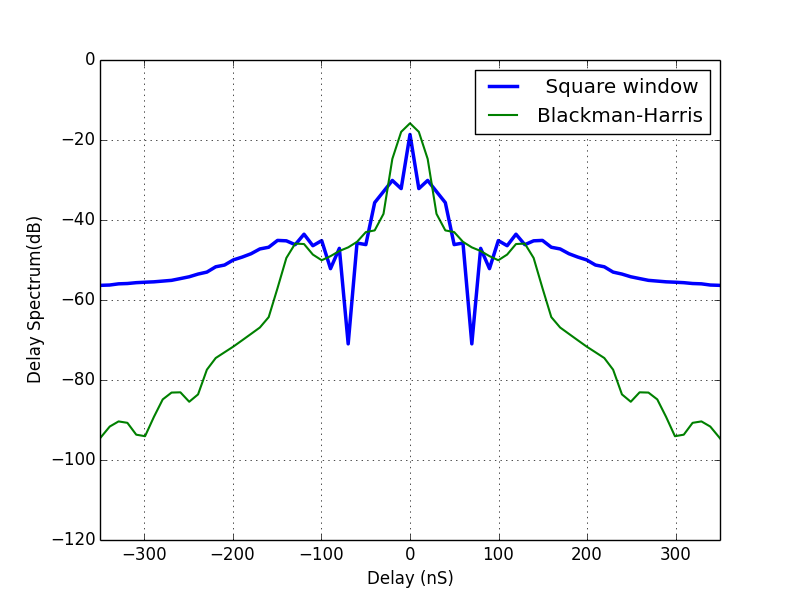
\includegraphics[width=\linewidth]{plots/window_effect.png}
\caption{Effect of finite bandwidth on estimation of delay spectrum: Blue line shows the delay spectrum of the HERA element computed from the measured data which is band limited between 100 to 200MHz. Green line shows the delay spectrum estimated from the same data set after multiplying the data by a Blackman Harris window. The delay spectrum of the windowed data set shows significant reduction in the instrument response at higher delays.}
\label{fig:window}
\end{figure} 

\subsection{\textbf{Multiple reflection between the feed and the backend.}}
Multiple reflections of the sky signal between the feed and the dish broadens the delay response of the instrument resulting in spill over of the smooth foreground power sky at higher delays. Another effect that have exact similar impact on the delay spectrum is the multiple reflection of the received signal between the feed output and the input of the analog backend and correlators. In our measurements, the feed output is connected to the VNA via a 50 feet long LMR 400 cable. This length correspond to a delay of $\approx 120~nS$ for the signals travelling through the cable. The delay spectrum of both feed and feed-dish assembly shows an enhanced feature at this delay indicating a reflection from the VNA input. We measure the VNA input reflections by disconnecting the feed and connecting an open load at the feed input of the cable. The measured return loss is shown in the figure \ref{fig:open_RL}. Since the electromagnetic wave travelling through a transmission line undergoes a $100\%$ reflections from an open ended transmission line, we compute the combined effect of the VNA input return loss along with the cable resistive loss from this measurement as shown in fiigure \ref{VNA_RL}. This results an important system design criterion for HERA. The VNA input return loss is found to be at a level of $-14$ to $-30dB$ across the measurement band. This is consistent with the matched provided by the commercially available RF connectors that are commonly used. This manifests itself in a peak in the delay spectrum which is $50~dB$ above the measurement noise floor. The delays at which this effect becomes dominant depends on the length of the cable. Due to finite return loss at the input of the backends, this effect will be present in all the observations and thus would impact the instrument delay spectrum. However, its effect could be reduced below the level where the foreground  achieving a return loss at the backend input is greater than at least $-30~dB$. 

\begin{figure*}[ht]
\begin{minipage}[b]{0.5\linewidth}
\centering
\includegraphics[angle=0, width=\linewidth]{plots/open_RL.png}
\end{minipage}
\hspace{0.1cm}
\begin{minipage}[b]{0.5\linewidth}
\centering
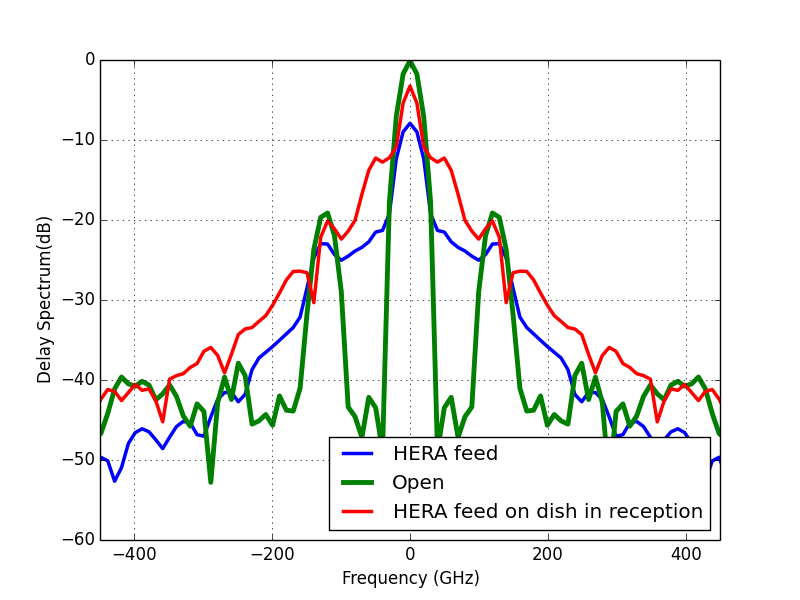
\includegraphics[angle=0, width=\linewidth]{plots/open_delay.png}
\end{minipage}
\caption{Left: Magnitude and phase of the return loss measured when the open load is connected at the feed input of the cable. Ideally, for an open load, the electromagnetic wave travelling through the transmission cable undergoes a $100\%$ reflections and magnitude of the return loss is $0dB$. However, due to the resistive loss in the cable, the a small part of the signal is dissipated in the cable resulting a smaller return loss.  Right: Delay spectrum of the open load that shows the multiple reflections at the VNA input. The delay spectrum of the feed and the feed-dish assembly is also plotted for comparison.}
\label{fig:open_RL}       
\end{figure*}

While measuring the return loss of the dish-feed assembly, the signal transmitted by the VNA is reflected first off the feed. This is represented by $\Gamma_{f}$ in equation \ref{eq:power_ratio}. This essentially represents a mismatched impedance between the feed and the 50 Ohm transmission line. In the delay domain, this appears at the zero delay bin. This response is identical whether or not the feed is suspended on the dish. We can, therefore, quantify this response by measuring the feed return loss while the feed is kept on the ground facing the sky. This results in a feed return loss including the surrounding cage structure but excluding the dish response. While a fraction, $\Gamma_{f}$, of the power is reflected off the feed, $1+\Gamma_{f}$ gets transmitted. In the receiving mode, upon initial incidence, $\Gamma_{f}$ of the voltage is reflected back into free space while $1+\Gamma_{f}$ enters the feed, and, in the delay domain, this appears at the zero delay bin. Using the return loss measurement of the feed $(\Gamma_{f})$ and the return loss measurement, $s_{11}$, of the dish, the feed assembly is corrected via equation \ref{eq:power_ratio} for the zero delay component, and the quantity of interest ${I_{rec}\over I_{sky}}$ is estimated. 
%
%
\begin{figure}
\centering
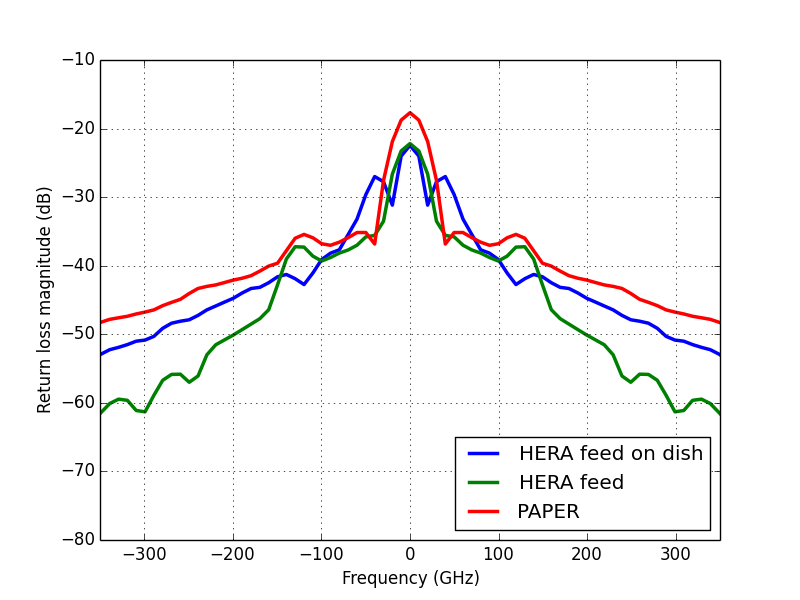
\includegraphics[width=\linewidth]{plots/delay_spectrum_100_200_BH.png}
\caption{Delay spectrum of the HERA element, the PAPER element, and the HERA feed estimated by taking the Fourier transform of the measured return loss of power at the feed output. The HERA feed design is driven by the PAPER element with an improved response at all delays. The feed, when suspended on the dish, results in a more complex return loss, and the corresponding delay response is shown in the figure.} %Delay units are incorrect!!!! Should be ns not GHz!!!!
\label{fig:delay_spectrum}
\end{figure}

\section{\textbf{Effect of instrument delay spectrum on 21cm power spectrum measurements}}



\begin{itemize}
\item 
\textbf{Comparison with electromagnetic simulation:}\\



The delay spectrum estimated from the simulated and measured return loss is shown in the figure \ref{fig:sim_em}. The two delay spectrum are in good agreement with each other upto around $60~ns$ up to which the structures in the delay domain are mostly caused due to signal reflections in the feed structure. Since the simulated return loss shows a better match of the antenna to the 50 Ohm transmission line. At zero delay , in case of simulation, almost $100\%$ of the sky signal is received whereas in case of measurements, this match is found to be less than $5~dB$ resulting in partial coupling of the sky signal to the system. Given all the reflections unaltered, if the matching in between the feed and the transmission line is improved by about $10~dB$, which is achievable in reality, the delay spectrum would improve substantially. This is plotted in grey. The work is currently under progress to improve the feed return loss at least by  $10dB$ (Eloy et al 2016 in prep?). Beyond $60~nS$ other multiple reflections manifests themselves at higher delays and the delay spectrum of the measurement and simulations begin to deviate from each other.

\begin{figure}
\centering
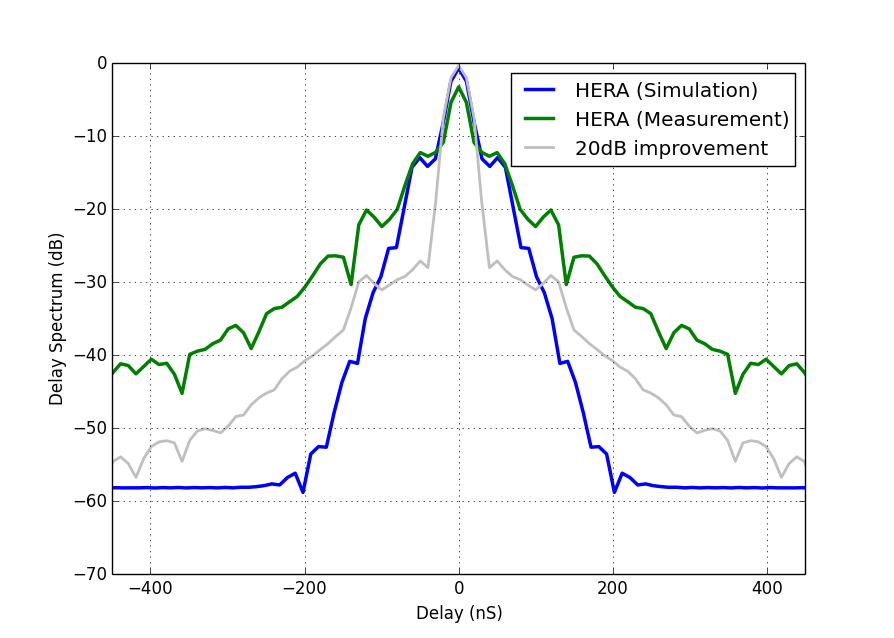
\includegraphics[width=\linewidth]{plots/delay_sim_meas.png}
\caption{Comparison between delay spectrum of HERA element estimated from the electromagnetic simulation of the feed return loss (dave deBoer 2016) and measurements by a vector network analyser.}
\label{fig:sim_em}
\end{figure}

\item
\textbf{Comparison with time domain simulation: }\\
In a related series of papers, (Ewall-Wice et al 2016) has shown the simulated power kernel of the HERA element which considers the electromagnetic simulations of the HERA feed and multiple reflection in between the dish and the feed vertex. Our measurements, in comparison to the simulations, shows a much complex structure in the delay spectrum. This results from various multiple reflections within and around the feed as well as in the cable connecting the feed output to the vector network analyser. Once again, keeping all other reflections within the system unchanged, a simple $~10dB$ improvement in the feed impedance match could match the simulations with measurements. 


\begin{figure}
\centering
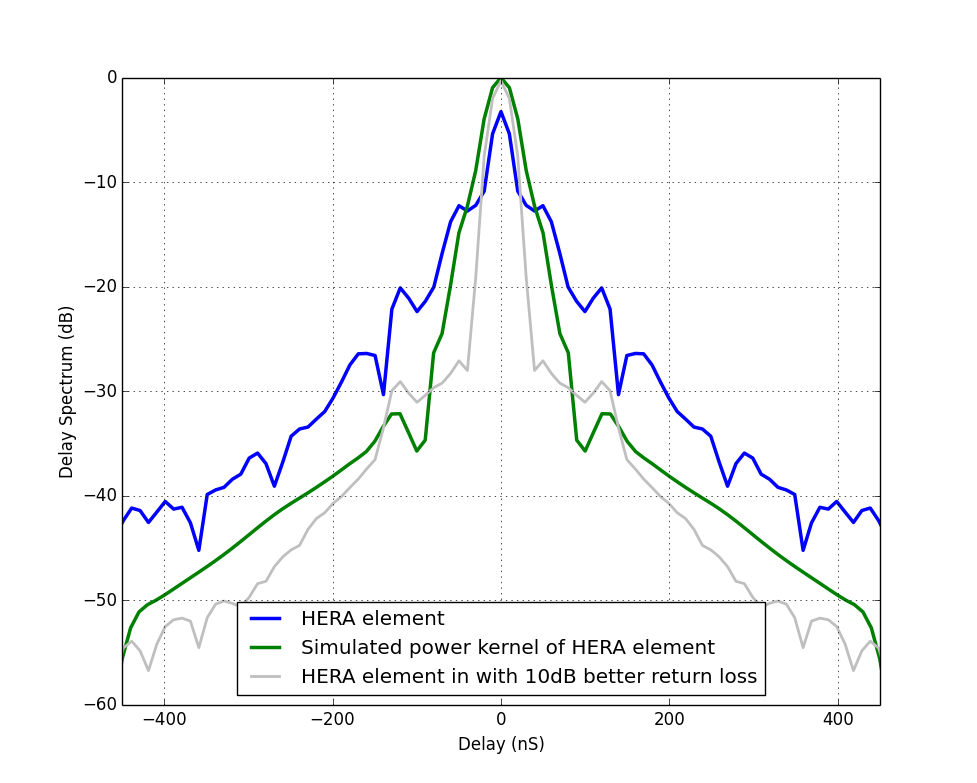
\includegraphics[width=\linewidth]{plots/delay_power.png}
\caption{Comparison between delay spectrum of HERA element estimated from the simulation of the multiple reflections between the feed and the dish and reflectometry measurements by a vector network analyser.}
\label{fig:sim_pk}
\end{figure}




\item
\textbf{Comparison with foreground simulation}
In a related series of papers, (Thyagarajan et al 2016) has presented the detailed sensitivity calculations of HERA is using a comprehensive foreground as well as model for EoR power spectrum for various simulated antenna element response. The theoretical limits for the level of signal attenuation required in order to reduce the foreground contaminations at the delay modes significant for power spectrum measurements are shown for three different lower limits of $k_\parallel$ values. The requirements for the reduced instrument response at higher delays are more stringent for the detection of lower $k_\parallel$ modes. The response is computed for the redshift of $z=8.47$ at frequency $150~MHz$. The yellow and cyan curves shows the improvement on the instrument delay spectrum that could be achieved by improving the feed return loss by $20, 30db$ respectively. With a $30dB$ improvement in return loss, for power spectrum at $k_{\parallel}>0.15$, the foreground contaminations at higher delays could potentially be limited to only a few delay modes. Achieving a $30~dB$ improvement at the feed is extremely challenging. However, since multiple reflections results in multiplication of the feed return loss as well as the input return loss at the backend, a $20~dB$ improvement in the feed and another $~20dB$ improvement in the mismatch between the cable and the backend input could establish the same. 

\begin{figure}
\centering
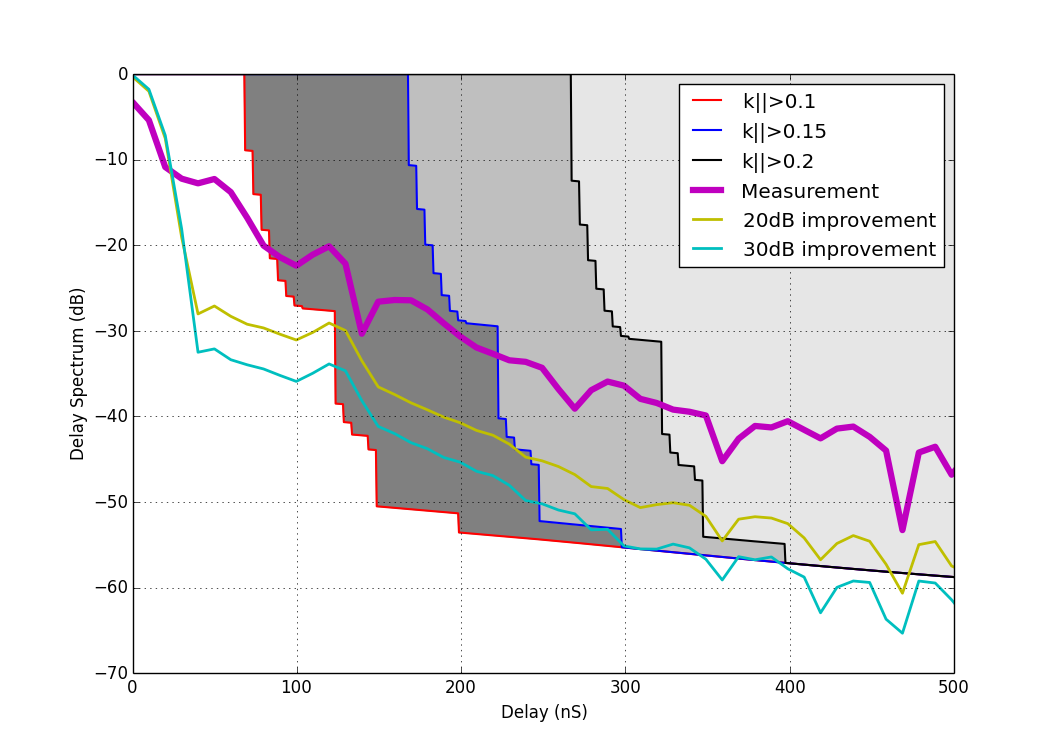
\includegraphics[width=\linewidth]{plots/meas_forground.png}
\caption{Delay spectrum of HERA element estimated from the reflectometry measurements by a vector network analyser compared to the limits of foreground simulation (Thyagarajan et al).}
\label{fig:sim_fg}
\end{figure}

\end{itemize}

\subsubsection{\textbf{Comparison of performance of HERA with PAPER}}
While PAPER has established the till date the most stringent upper limit on the 21cm power spectrum measurement, the need to increase the measurement sensitivity called for increased collecting area per PAPER antenna. This has driven to the parabolic reflector antenna based design of the PAPER successor HERA where essentially the PAPER antenna with minor modification of the ground plane-side plane assembly works as the feed and thus having larger collecting area per element. Figure \ref{fig:freq} shows the return loss measurement of power of the PAPER antenna and figure \ref{fig:delay_spectrum} shows (red line) the corresponding delay spectrum. The feed element shows improved delay response compared to the PAPER element across all delays $>50~ns$ with marginal improvement at delays $<50~ns$. The delay response of the HERA element degrades marginally as the feed is suspended over the dish due to multiple reflections between the feed and the dish.  It is evident that majority of the response at lower delays are contributed due to the feed and its supporting structure at lower delays which is somewhat common to all three measurements. At the lower delays, the structures in the delay response remains unaltered even with the variation of the feed height relative to the dish vertex. It is essentially these structures set lower limits on the $k_{||}$ that could be probed and any redshift $z$ above the instrument footprint. 

%\section{\textbf{Effect of instrument delay spectrum on 21cm power spectrum measurements} }
%The delay response of the instrument is dependent on the band chosen for the Fourier transform.
%The measurement bandwidth effects the amplitude and phase of the delay spectrum. Fourier transforms taken over wider bandwidth
%become dominated by the feed sidelobes outside the operating band, making the resultant delay profiles less relevant
%for the power spectrum performance of the HERA instrument.  Conversely, when performing Fourier transforms over much 
%narrow bands (the windowed $20MHz$ bands typical of PAPER analysis), the width of the resulting delay profile
%becomes dominated by sidelobes of low delay emission interacting with the narrow bandwidth kernel.  
%Although this may appear to be a relevant performance metric for PAPER power spectrum analysis, such an analysis typically pre-filters out low-delay emission using wide bandwidths precisely to avoid sidelobes from low-delay emission.  Hence, the most relevant delay-spectrum performance profile is that taken using the $100-200MHz$ band. \textbf{In the $100-200MHz$ delay profile, we see a delay response of $-25dB$ at $60ns$, which slopes down to $-60dB$ at $\sim120ns$.  WRITE AGAIN}


%Figure \ref{fig:elevator} is again a delay plot of the return loss at four different feed suspension heights. 
%We use the PAPER bandwidth and note
%that the measurements are near identical at low delays, implying that low delay reflections are caused primarily by reflections within the feed cage. 
%However, at higher delays we notice discrepancies between the different heights.
%In addition, Figure \ref{fig:outofthedish} presents measurements taken of the feed only.away from the dish. Echosorb is placed under the feed for some of the
%measurements, with the expectation that it will prevent any reflections off the
%ground.
% Measurements are also taken of the feed inside its metal cage in various configurations. It is shown that the feed performs best without the cage and with the absorber. 
%All these measurements are suggestive of the  fact that the feed-cage assembly itself is responsible for a significant portion of the structure up to $60ns$ and
%that the cylindrical cage may be contributing up to $20ns$ to the width of the delay profile. 
%We note that this depends stronglyon its coupling to structures around it. 
%Structure beyond $60ns$ appears to scale with the height of the feed above the dish.



\section{\textbf{Conclusion}}

The delay-domain performance of the HERA dish is central to HERA's function as a power spectrum instrument.
As we have seen, reflectometry measurements can help characterize HERA's performance in this domain, and
as Equation \ref{eqn:ratio1} shows, these measurements must be adjusted for a difference in transmission/reflection
at the first feed encounter in order to be interpreted as the delay response of a feed relative to an incident
plane wave from the sky.  We also see that the choice of windowing function is critical for accurately measuring the
antenna delay response at higher delays, where sidelobes from much higher amplitude responses at small delays can easily
dominate.  We find Hamming, Hanning, and Blackman-Harris windows to be generally adequate while square windowing functions are not.
Given the critical nature of the windowing function, we recommend that all reflectometry measurements be performed in the
frequency domain, so that the data could be Fourier transformed with the appropriate window.

Taken all together, we summarize that the first version of the HERA dish, with a PAPER-style feed and cylindrical cage, is close to meeting
specification, but will require additional work to fall below $-60dB$ at $60ns$.  Given that the width of the delay response is a convolution
of the feed response and the dish reflections, it is not possible to perfectly decouple the response of the feed from that of the dish.
It may be possible to achieve enough of a reduction to meet specification by modifying the feed.
Given that previous measurements using a PAPER feed with a simple backplane exhibit structure above $-60dB$ at $60ns$,
we deduce that these advances will most likely require improving the feed return loss.  We also recommend re-investigating the scattering
cone for reducing standing waves between the feed and dish.  Finally, given the proximity of our measurements to the rough 
specification that was adopted for 
HERA of $-60dB$ attenuation at $60ns$, we recommend reinvestigating this specification to determine more accurately the impact of 
the element's current delay performance on HERA science.  We suspect that, at the level of $-50dB$ at $60ns$ and $-60dB$ at $120ns$, this
performance may indeed be adequate for the delay-domain power spectrum analysis for which HERA has been optimized.

%\bibliography{biblio}{}
\bibliography{Reference}{}
\bibliographystyle{apj}
\end{document}

